\documentclass[ngerman,hyperref={pdfpagelabels=false}]{beamer}

% -----------------------------------------------------------------------------

\graphicspath{{images/}}

% -----------------------------------------------------------------------------

\usetheme{KIT}

\setbeamercovered{transparent}
%\setbeamertemplate{enumerate items}[ball]

\newenvironment<>{KITtestblock}[2][]
{\begin{KITcolblock}<#1>{#2}{KITblack15}{KITblack50}}
{\end{KITcolblock}}

\usepackage[ngerman,english]{babel}
\usepackage[utf8]{inputenc}
\usepackage[TS1,T1]{fontenc}
\usepackage{array}
\usepackage{multicol}
\usepackage[absolute,overlay]{textpos}
\usepackage{beamerKITdefs}

\pdfpageattr {/Group << /S /Transparency /I true /CS /DeviceRGB>>}	%required to prevent color shifting withd transparent images


\title{Algorithmen I - Tutorium 12}
\subtitle{Sebastian Schmidt -- \textit{isibboi@gmail.com}}

\author[Sebastian Schmidt]{Sebastian Schmidt}
\institute{Arbeitsgruppe Kryptographie und Sicherheit}

\TitleImage[width=\titleimagewd,height=\titleimageht]{titel}

\KITinstitute{Arbeitsgruppe Kryptographie und Sicherheit}
\KITfaculty{Fakult\"at f\"ur Informatik}

% -----------------------------------------------------------------------------

\begin{document}
\setlength\textheight{7cm} %required for correct vertical alignment, if [t] is not used as documentclass parameter


% title frame
\begin{frame}
  \maketitle
\end{frame}

\begin{frame}{Erinnerung Kruskal}
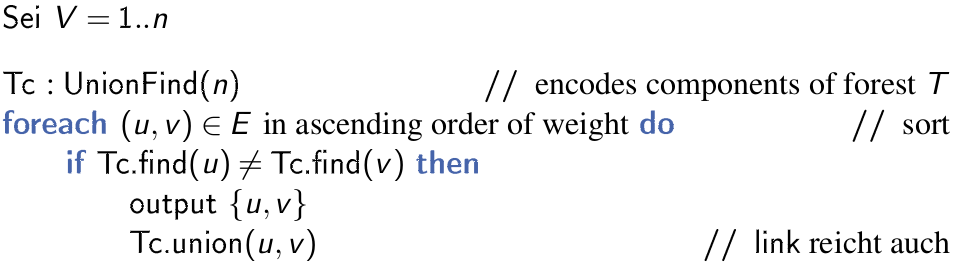
\includegraphics[width=\textwidth]{k}
\end{frame}

\begin{frame}{Union-Find}
Struktur: Array

Operationen: \texttt{union(i, j)}, \texttt{find(i)}
\end{frame}

\begin{frame}{Greedy-Algorithmen}
Was sind Greedy-Algorithmen?

Beispiele?
\end{frame}

\begin{frame}{Vertex Cover}
Gegeben Graph $G$.

Finde minimale Menge $V' \subseteq V$ mit $\forall (u, v) \in E: {u, v} \cap V' = \emptyset$.


\vspace{2em}
Formuliere Vertex Cover als ILP.
\end{frame}

\begin{frame}{Linear Program}
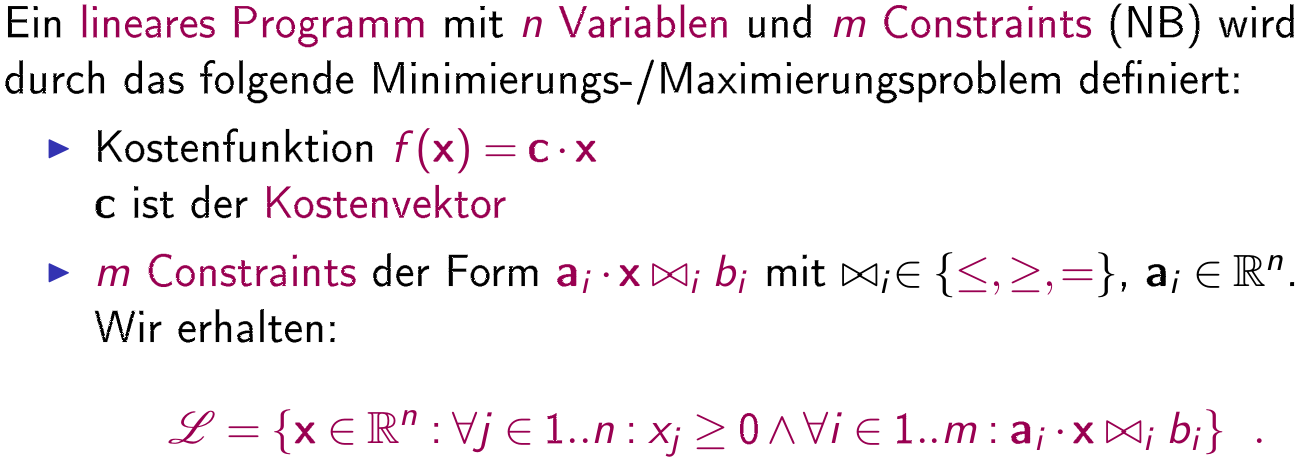
\includegraphics[width=\textwidth]{LP}
\end{frame}

\end{document}